\documentclass{article}

% if you need to pass options to natbib, use, e.g.:
% \PassOptionsToPackage{numbers, compress}{natbib}
% before loading nips_2018

% ready for submission
\usepackage[final]{corl_2018}

% to compile a preprint version, e.g., for submission to arXiv, add
% add the [preprint] option:
% \usepackage[preprint]{nips_2018}

% to compile a camera-ready version, add the [final] option, e.g.:
% \usepackage[final]{nips_2018}

% to avoid loading the natbib package, add option nonatbib:
% \usepackage[nonatbib]{nips_2018}

\usepackage[utf8]{inputenc} % allow utf-8 input
\usepackage[T1]{fontenc}    % use 8-bit T1 fonts
\usepackage{hyperref}       % hyperlinks
\usepackage{url}            % simple URL typesetting
\usepackage{booktabs}       % professional-quality tables
\usepackage{amsfonts}       % blackboard math symbols
\usepackage{amsmath}       % blackboard math symbols
\usepackage{amssymb}       % blackboard math symbols
\usepackage{nicefrac}       % compact symbols for 1/2, etc.
\usepackage{microtype}      % microtypography
\usepackage{color}
\usepackage{natbib}
\usepackage{algpseudocode,algorithm,algorithmicx}
\usepackage{comment}

\usepackage{graphicx}
\graphicspath{{figures/}}

\usepackage{tikz}
\usepackage{pgffor}
\usetikzlibrary{arrows,positioning}

% My commands
\newcommand{\R}{\mathbb{R}}
\newcommand{\E}{\mathbb{E}}
%\newcommand{\TODO}[1]{\textcolor{red}{\textbf{TODO: #1}}}
\newcommand{\TODO}[1]{}

\newcommand{\cA}{\mathcal{A}}
\newcommand{\cH}{\mathcal{H}}
\newcommand{\cL}{\mathcal{L}}
\newcommand{\cN}{\mathcal{N}}
\newcommand{\cO}{\mathcal{O}}
\newcommand{\cS}{\mathcal{S}}
\DeclareMathOperator*{\argmax}{argmax}

\newcommand{\blind}{\emph{blind}}
\newcommand{\plain}{\emph{plain}}
\newcommand{\extra}{\emph{extra}}
\newcommand{\embed}{\emph{embed}}
\newcommand{\traj}{\emph{traj}}
\newcommand{\embedfn}{e}
\newcommand{\idfn}{id}
\newcommand{\latent}{\cL}

\newcommand{\secref}[1]{Section \ref{#1}}
\newcommand{\figref}[1]{Figure \ref{#1}}
\newcommand{\tabref}[1]{Table \ref{#1}}


\title{Learning an abstract system identification space for adaptive online control}

% The \author macro works with any number of authors. There are two
% commands used to separate the names and addresses of multiple
% authors: \And and \AND.
%
% Using \And between authors leaves it to LaTeX to determine where to
% break the lines. Using \AND forces a line break at that point. So,
% if LaTeX puts 3 of 4 authors names on the first line, and the last
% on the second line, try using \AND instead of \And before the third
% author name.

\author{
  James A.~Preiss \\
  Department of Computer Science\\
  University of Southern California\\
  Los Angeles, CA 90089\\
  \texttt{japreiss@usc.edu} \\
  %% examples of more authors
  \And
  Karol Hausman \\
  Google Brain \\
  <TODO: what address?> \\
  \texttt{TODO: google brain email?} \\
  \AND
  Gaurav S. Sukhatme \\
  Department of Computer Science\\
  University of Southern California\\
  Los Angeles, CA 90089\\
  \texttt{gaurav@usc.edu} \\
  %% Coauthor \\
  %% Affiliation \\
  %% Address \\
  %% \texttt{email} \\
  %% \And
  %% Coauthor \\
  %% Affiliation \\
  %% Address \\
  %% \texttt{email} \\
  %% \And
  %% Coauthor \\
  %% Affiliation \\
  %% Address \\
  %% \texttt{email} \\
}


\begin{document}

\maketitle

\begin{abstract}
\end{abstract}

\section{Introduction}

Reinforcement learning (RL) is a highly general framework for learning policies that make decisions sequentially in an environment.
RL is a compelling approach to robotic control problems
because the same learning algorithm and policy structure can be applied to a wide range of robot environments
without requiring per-environment manual effort or insight.
Yet, in contrast to the generality of RL itself,
the policies trained with RL are usually highly specialized and fail to generalize to other similar environments,
even when the differences are small~\citep{zhang-study-on-overfitting}.

Overfitting to the training environment is problematic if we desire to deploy a trained policy on other systems.
Training in a fast simulator and deploying on a real robot can save lots of time,
but simulators cannot faithfully reproduce every detail of physical phenomena such as fluid dynamics or collision and friction forces.
If a robot manufacturer wishes to train a policy in a lab and deploy it on mass-produced robots,
they must account for manufacturing variations that will affect dynamics.

Failure to generalize has been the subject of intense attention from the RL community.
Domain randomization of dynamics parameters~\citep{antonova-pivoting-corr17, zhu-RL-IL-diverse}
or visual attributes~\citep{sadeghi-cad2rl-rss17,tobin-domainrand-arxiv17,james-domain-xfer}
has demonstrated surprisingly good generalization ability without changes to the policy class or learning algorithm.
Related approaches include ensembles of policies~\citep{actor-mimic,teh-distral},
adversarial perturbations of state or observations~\citep{pinto-robust-adversarial-RL,huang-adversarial-attacks},
and learning robust feature spaces~\citet{higgins-DARLA,bousmalis-domainseparation-nips16}.
Fine-tuning or progressive networks~\citet{rusu-progressive-nets} \TODO{fine-tuning citation}
use a policy trained in simulation as a starting point for further learning in the test environment.
Model-agnostic meta-learning (MAML)~\citep{finn-maml-icml17}
explicitly prepares for the fine-tuning by unrolling the policy gradient update in the training objective.
\TODO{end this paragraph.}

In this paper, we focus on scenarios where the variation in dynamics parameters
is large enough to impede domain randomization,
but small enough that updating the parameters of the policy at test time is not strictly necessary.
We introduce an architecture and training regime that produce a policy
that can adapt online in real time to a test system with unknown dynamics parameters.
Our framework is inspired by control theoretic architectures for online system identification
similar to~\citet{yu-up-osi-rss17},
but instead of attempting to identify the true parameters of the system,
we learn an abstract embedding space that is both
1) useful to help the policy behave optimally, and
2) easy to identify from a short state-action trajectory.
\citet{peng-dynamics-randomization-corr17} also avoid estimating the true parameters by using a recurrent policy,
but our architecture makes it possible to explicitly encourage behavior that makes system identification easy
in the RL reward.
We demonstrate experimentally that our learned embeddings can perform dimensionality reduction on unobservable subspaces of the dynamics parameters,
and separate nearby parameter values that require disjoint behavior styles.

\section{Related Work}
Work addressing RL generalization generally fall into one of two categories:
those that attempt to improve the \emph{a priori} generalization performance of the policy without any data from the test environment,
and those that update the parameters of the control policy \emph{a posteriori} after collecting some data from the test environment,
or while training in both environments simultaneously.

The most straightforward \emph{a priori} approach is domain randomization,
in which the parameters of the dynamics and/or observations are randomized during training,
but the final policy does not explicitly perform system identification at test time.
%
Randomization of dynamics parameters in simulation has been shown to increase generalization ability~\citep{antonova-pivoting-corr17, zhu-RL-IL-diverse}.
Random textures and colors in the visual input has been used for successful sim-to-real transfer
for indoor quadrotor navigation~\citep{sadeghi-cad2rl-rss17}
and simple manipulation tasks~\citep{tobin-domainrand-arxiv17,james-domain-xfer}.
These methods focus on the visual part of the problem and use higher-level control inputs
to abstract away physical details of the target system.
Ensemble approaches optimize for mean performance over a set of models~\citep{mordatch-ensemble-icra15}
or distill a set of expert policies into a single policy that performs well in all environments~\citep{actor-mimic,teh-distral}.

Domain randomization has performed well in the literature and in our own experiments.
However, domain randomization implicitly assumes that, given the observable states of the system,
there exists an action that will produce acceptable behavior over all possible values of the hidden, randomized states.
This assumption may not hold if the set of possible target environments is diverse.

Other \emph{a priori} approaches include adversarial setups,
where a learned ``antagonist'' agent attempts to decrease the primary ``protagonist'' agent's reward
by injecting physical disturbances into the system~\citep{pinto-robust-adversarial-RL}
or perturbing the observation input in vision-based agents~\citep{huang-adversarial-attacks}.
\citet{higgins-DARLA} build a factorized generative model of the visual scene
and train the agent on this space instead of pixel inputs.


The \emph{a posteriori} approach has been widely deployed in visual domains
using generative adversarial networks (GANs) in the single-direction~\citep{bousmalis-domain-gan-cvpr17}
and cycle-gan cases~(\TODO{cite})
or by learning a domain-invariant feature space~\citep{bousmalis-domainseparation-nips16}.

\citet{christiano-deep-inverse-dynamics-corr16} learn an inverse dynamics model and use the trained policy in the simulator to select desired states.
\TODO{characterize better.}

\citet{rajeswaran-epopt-corr16} blended the two categories by introducing
modifications to the training approach for blind policies
\TODO{introduce terminology for ``blind'' policies}
to adapt the simulated parameter distribution based on data from interacting with the target domain
and to focus the training objective on those parameters where the policy performs worst.
\TODO{run-on sentence}


\citet{rusu-progressive-nets} deploy the \emph{progressive nets} framework
where additional cross-connected layers are added to a neural network
for sim-to-real transfer.

In cases where this assumption is violated, the policy must be able to behave differently in different environments,
and there must be a mechanism to extract some information about the hidden parameters of the environment during interaction.
This is the scenario considered in this paper.
A similar approach to ours is~\citet{yu-up-osi-rss17},
where the authors trained a policy that takes the dynamics parameters as input
and an online system identification module to estimate them.
We observe that estimating the true dynamics parameters is more work than needed--
we can instead learn to map the dynamics parameters into an embedding space
that is more useful for the policy, as well as being easier to estimate.
~\citet{peng-dynamics-randomization-corr17} make a similar observation and use a recurrent policy architecture.
A recurrent architecture is able to extract information about the environment in its internal state without imposing any particular structure on the information that is extracted.
By comparison, our framework makes it possible to modify the training reward such that the model is explicitly encouraged to behave in a manner that makes the parameters easily observable.

Model-agnostic meta-learning (MAML)~\citep{finn-maml-icml17} is a hybrid of \emph{a priori} and \emph{a posteriori} approaches.
MAML incorporates the policy gradient update step directly in its training objective,
optimizing the policy for adapting to the test environment in a single gradient descent step after gathering a small amount of data.
\citet{clavera-maml-model} apply a similar framework to model-based RL, training a meta-model in simulation
to update rapidly after gathering few real-world trajectories.




\section{Problem statement}

We consider reinforcement learning in a Markov Decision Process (MDP)
%where $\cS \subseteq \R^\cS$ is the state space,
%$\cA \subseteq \R^\cA$ is the action space,
%$p : \cS \times \cA \times \cS \mapsto \R_{\geq 0}$ are the stochastic dynamics,
%$\rho : \cS \mapsto \R_{\geq 0}$ is the initial state distribution,
%and $r : \cS \times \cA \mapsto \R$ is the task reward function.
with state space $\cS$,
action space $\cA$,
stochastic dynamics $p : \cS \times \cA \times \cS \mapsto \R_{\geq 0}$,
initial state distribution $\rho : \cS \mapsto \R_{\geq 0}$,
task reward function $r : \cS \times \cA \mapsto \R$,
and finite time horizon $H \in \mathbb{N}$.
The state space $\cS$ is partitioned into
the task space $\cS_T$
and the dynamics space $\cS_D$, such that $\cS = \cS_T \times \cS_D$.
The task space $\cS_T$ consists of the intrinsic state of the robot, such as the angles and angular velocities of revolute joints, as well as task specification inputs such as a goal position.
These states can be measured or accurately estimated in the real system.
The dynamics space $\cS_D$ consists of parameters such as joint geometries, moments of inertia, sensor and actuator characteristics, and coefficients of drag or friction.
These parameters may be unmeasurable or difficult to estimate.
We seek to learn a stochastic policy maximizing the expected reward over all dynamics parameters:
\begin{equation}\begin{split}
\pi : \cS \times \cA \mapsto \R_{\geq 0}, \quad
\pi^\star = \argmax_\pi \E_{s_d \in \cS_D} \sum_{t = 0}^H
r(s_t, a_t).
\label{objective}
\end{split}\end{equation}
While training in the simulator, we assume that we have access to the ground truth system identification parameters $s_d$.
However, when testing, the true system identification parameters are unknown.
%Due to the complexity and nonlinearity of real-world dynamics,
%small errors in the measurements of these states can result in major differences between the behavior of the system in reality and in simulation.

\section{Framework}
A natural approach to the problem~\eqref{objective}, explored by~\citet{yu-up-osi-rss17}, is to learn a function to estimate $s_d$ from a state-action trajectory $\tau = (s_1, a_1), (s_2, a_2), \dots, (s_k, a_k)$.
At test time, we could replace the system identification portion of the policy input
with the output of the learned state estimator.
However, this approach presents two problems.

First, it requires estimating every system identification parameter,
even though some may be difficult to estimate or redundant.
For example, it may be possible to reduce a mass and an acutator force limit into a single dimensionless quantity.
An example of this issue is shown in \secref{pointmass}.
Reductions such as these can make the estimation problem easier, but they may not be easy to derive by hand on complex systems.

Second, the behavior that maximizes the expected reward~\eqref{objective}
in simulation with known $s_d$ may not be the best behavior for making the state estimation task easier.
It is preferable to learn a behavior that balances the primary objective~\eqref{objective}
with a secondary objective of making the state estimation task as easy as possible.

In this work, we present a framework that addresses both of these concerns.
We introduce a learned function $\embedfn : \cS_D \mapsto \latent$
that maps the system identification parameters to an abstract latent space $\latent$.
We then learn a function $\idfn : (\cS \times \cA)^k \mapsto \latent$, for $1 < k \ll H$,
that attempts to recover the value of the latent space by observing a state-action trajectory.
The functions $\embedfn$ and $\idfn$ are learned simultaneously with the policy $\pi$.
The latent space creates an opportunity to distill the full complexity of the system identification space $\cS_D$ into a space that is potentially more useful for the policy to produce optimal behavior,
while simultaneously being easier to estimate.

While the latent space may help make the system identification task easier,
it has a failure mode that must be considered:
if $\embedfn$ and $\idfn$ both map to the same constant value for any input,
$\idfn$ will achieve perfect performance during training,
but the embedding will not influence the policy, and $\pi$ will be reduced to a ``lowest common denominator'' policy.
To avoid this problem, we impose a structure where the parameters of the embedding function $e$
can only be learned via the RL objective, which includes a term rewarding accurate state estimation of $id$:
\begin{equation}\begin{split}
\pi^\star &= \argmax_\pi \E_{s_d \in \cS_D} \sum_{t = 0}^H \gamma^t r(s_t, a_t) \\
&+ \alpha_{id} \E_{\tau \sim \text{\TODO{complicated}}} \| id(\tau) - e(s_d) \|_2 \\
&+ \alpha_{\cH}\cH(\pi) \\
&+ \alpha_{KL} KL(e(s_d), \cN(0,1))
\label{objective-full}
\end{split}\end{equation}
In the modified objective~\eqref{objective-full},
we emphasize that the $\alpha_{id}$ term is part of the reinforcement learning reward
for the policy $\pi$.
We also add entropy regularization to the policy $\pi$ to stabilize the use of stochastic policy gradient RL algorithms,
and a KL divergence term encouraging the distribution of the embeddings
to match the first two moments of the unit normal distribution.
The latter ensures that the supervised learning data sets presented to the identification function $id$ do not require any separate whitening step.
\TODO{better motivation? It also helps avoid the collapse to a constant function,
but technically we already ``solve'' that by adding the estimation loss to the RL objective...}

The state estimation function $id$ is not updated by the RL algorithm.
It is updated in a separate supervised learning step, performed after each iteration of RL.
In our experiments, $id$ takes the form of a one-dimensional convolutional neural network
with trajectory length of $k = 16$.
Details of the architecture are given in~\secref{implementation}.
The convolutional architecture is chosen to allow longer trajectory inputs
without requiring a large number of parameters.
Additionally, it matches the intuition that differentiation and/or integration of the state and action trajectories
is often required to estimate the underlying dynamics parameters \TODO{cite?}.

\begin{comment}
\begin{table}[h]
\centering
\begin{tabular}{lll}
Type     & Filters & Size \\
\hline
Input    & --           & dim($\cS \times \cA$) \\
Conv1D   & 32           & 3 \\
Conv1D   & 32           & 3 \\
ReLu     & --           & -- \\
Max Pool & --           & 2 \\
Conv1D   & 32           & 5 \\
ReLu     & --           & -- \\
Linear   & dim($\cL$)   & -- \\
\end{tabular}
\caption{Architecture of 1D convolutional neural network used to learn the embedding estimator $id$.}
\label{conv1d}
\end{table}
\end{comment}



\begin{algorithm}[h]
\caption{\TODO{Name our method.}}
\begin{algorithmic}
\While{not converged}
  \State sample dynamics parameters $s_D^1,\ \dots,\ s_D^N$ uniformly from $\cS_D$
  \State collect rollouts $R$ and task rewards from $\pi$ for each of the $N$ parameters
  \State use SysID network $\idfn$ to estimate embedding $\hat e_D$ for sliding $k-$window over $R$
  \State update $\pi$ using on-policy RL for total reward $r = r_T + \alpha_{\cH}\cH(\pi) + \alpha_{ID} \E_{\pi} (\hat e_D - e_D(s_D))^2$
  \State update SysID network $\idfn$ using supervised learning
\EndWhile
\end{algorithmic}
\end{algorithm}


\section{Experiments}

\begin{figure}
\centering
\textbf{Training Time:}

\vspace{0.4cm}
\begin{tikzpicture}
\tikzstyle{box}=[draw=black, fill=white, inner sep=2mm, rounded corners=1mm]
\tikzstyle{bigbox}=[box, minimum height=1.6cm]
\tikzstyle{branch}=[circle,inner sep=0pt, minimum size=0.15cm, fill=black]
\tikzstyle{arrow}=[->]

\node[bigbox, align=center] (enviro) {Simulation \\ Environment};
\node[bigbox, align=center, right=1.75cm of enviro] (policy) {Policy \\ $\pi$};
\node[box, below=of enviro.south east, xshift=0.3cm] (embedder) {Embedder $\embedfn$};
\node[box, right=of policy, align=center] (traj)
{
  Trajectory $\tau$ \\
  \begin{tikzpicture}
  \foreach \offset in {1,...,5}
  {
    \node[box, sharp corners] (\offset) at (-0.05 * \offset, 0.1 * \offset) {$s_{t - 1},\ a_{t-1}$};
  }
  \end{tikzpicture}
};
\node[box, right=of traj] (estimator) {Estimator $\idfn$};
\node[box, below=0.65cm of traj, align=center] (sup-loss) {Supervised\\ Learning Loss};

\draw [arrow] ([yshift=0.4cm]enviro.east) -- node [above] {states} ([yshift=0.4cm]policy.west);
\draw [arrow] ([yshift=-0.4cm]policy.west) -- node [below] {actions} ([yshift=-0.4cm]enviro.east);
\draw [arrow] ([xshift=-0.5cm]enviro.south) |- node [pos=0.25, right] {SysID} (embedder.west);
\draw [arrow] (embedder.east) -| node [branch, label=below:{embeddings}] (embeds) {} (policy.south);
\draw [arrow] (traj) -- (estimator);
\draw [arrow] ([xshift=0.5cm]estimator.south) |- node [pos=0.35, left, align=right] {estimated\\embeddings} (embeds-|sup-loss.east);
\draw [arrow] (embeds) -- (embeds-|sup-loss.west);
\end{tikzpicture}

\vspace{0.8cm}

\textbf{Testing Time:}

\vspace{0.4cm}
\begin{tikzpicture}
\tikzstyle{box}=[draw=black, fill=white, inner sep=2mm, rounded corners=1mm]
\tikzstyle{bigbox}=[box, minimum height=1.6cm]
\tikzstyle{branch}=[circle,inner sep=0pt, minimum size=0.15cm, fill=black]
\tikzstyle{arrow}=[->]

\node[bigbox, align=center] (enviro) {Test \\ Environment};
\node[bigbox, align=center, right=1.75cm of enviro] (policy) {Policy \\ $\pi$};
\node[below=1.2cm of enviro.south east, xshift=-0.75cm, text=red, inner sep=0pt] (embedder) {$\times$};
\node[box, right=of policy, align=center] (traj)
{
  Trajectory $\tau$ \\
  \begin{tikzpicture}
  \foreach \offset in {1,...,5}
  {
    \node[box, sharp corners] (\offset) at (-0.05 * \offset, 0.1 * \offset) {$s_{t - 1},\ a_{t-1}$};
  }
  \end{tikzpicture}
};
\node[box, right=of traj] (estimator) {Estimator $\idfn$};
%\node[below=0.65cm of traj, align=center] (est-embed) {estimated\\ embeddings};

\draw [arrow] ([yshift=0.4cm]enviro.east) -- node [above] {states} ([yshift=0.4cm]policy.west);
\draw [arrow] ([yshift=-0.4cm]policy.west) -- node [below] {actions} ([yshift=-0.4cm]enviro.east);
\draw [draw=red, text=red] ([xshift=-0.5cm]enviro.south) |- node [pos=0.25, right] {SysID} (embedder.west);
%\draw [arrow] (embedder.east) -| node [branch, label=below:{embeddings}] (embeds) {} (policy.south);
\draw [arrow] (traj) -- (estimator);

%\draw [arrow] ([xshift=0.5cm]estimator.south) |- (est-embed);
%\draw [arrow] (est-embed) -| (policy.south);
\draw [arrow, draw=blue, text=blue] ([xshift=0.5cm]estimator.south) |- ++(0,-1.85cm) node [below=0.35cm of traj, align=center]{estimated\\embeddings}  -| (policy.south);

%\draw [arrow] (embeds) -- (embeds-|sup-loss.west);
\end{tikzpicture}
\vspace{0.4cm}
\caption{
Overview of experimental setup in this paper.
At training time, correct dynamics parameters are available from the simulator.
A mapping $\embedfn$ from parameters to an abstract embedding space is learned,
along with a module $\idfn$ to estimate the embedding value from a state-action trajectory $\tau$.
The policy is rewarded for behavior that improves estimation accuracy.
At testing time, the true dynamics parameters are no longer known,
and the estimated embeddings are input directly to the policy.
}
\label{fig:overview}
\end{figure}
In this section, we illustrate the desirable properties of the learned embedding space $\cL$
and compare the performance of our architecture (denoted \embed) against several baselines:
\begin{enumerate}
\item \blind: A ``blind'' policy that has no access to $\cS_D$ in any form, representing the domain randomization.
\item \plain: A policy conditioned on the true system identification parameters $\cS_D$ instead of the learned embedding.
\item \extra: Same as \plain, but with an extra fully connected layer between $\cS_D$ and $\pi$, such that the total number of policy parameters is equal to \embed.
%\item \traj: A policy where the state-action trajectory is input through a 1D convolutional network (identical to the SysID network) in training, without any condition that this network should estimate $\cS_D$ or an embedding.
\end{enumerate}
The structure of the experimental setup is shown in~\figref{fig:overview}.
The presented experimental results suggest that our embedding framework learns policies that generalize better than the alternatives \TODO{fingers crossed.}

\subsection{Point-Mass Environment}
\label{pointmass}
The point-mass environment serves as a ``simplest possible'' scenario to demonstrate our approach.
The state space is position and velocity in two dimensions.
The action space $a \in \cA = [-1, 1]^2$ is a bounded force in two dimensions.
The system identification space is a gain factor $g \in \pm[0.2, 2]$ \TODO{match code}.
such that the true force applied to the mass is $g \cdot a$.
The low dimensions of this system allow us to visualize the properties of the learned embedding more easily.
The system dynamics are:
\begin{equation}\begin{split}
\dot p = v, \quad \dot v = -\epsilon v + ga
\end{split}\end{equation}
where $0 < \epsilon \ll 1$ is a damping parameter.
The policy is trained to push the mass towards the origin
by the reward function $r = -\|p\|_1$.
%by the reward function $r = -\sqrt{|g|} \cdot \|p\|_1$,
%where the scaling factor $\sqrt{|g|}$ balances the rewards in the low- and high-gain scenarios
%based on the minimum-time bang-bang solution to the implied optimal control problem.
Due to the unknown sign of the gain factor, the ``blind'' policy cannot possibly perform well in this environment.
%\TODO{better explanation, avoid readers thinking it's too contrived}

%The point-mass learning curves are shown in \TODO{figure}.
%As expected, the \emph{blind} policy performs very poorly.
%The \emph{plain} and \emph{extra} policies perform in between.

\begin{comment}
\begin{table}
\centering
\begin{tabular}{l c c c c}
       &          & test         & reward $\sigma$          & reward $\sigma$       \\
flavor & $\alpha$ & reward $\mu$ &            (per-episode) &            (per-seed) \\
\hline
\blind & 0.1 & -80.3 & 27.6 & 2.6 \\
\plain & 0.1 & -70.8 & 28.2 & 2.4 \\
\extra & 0.1 & -67.1 & 34.6 & 2.7 \\
\embed & 0.1 & \textbf{-62.7} & 27.6 & 0.8 \\
\end{tabular}
\end{table}
\end{comment}

\begin{figure}
\centering
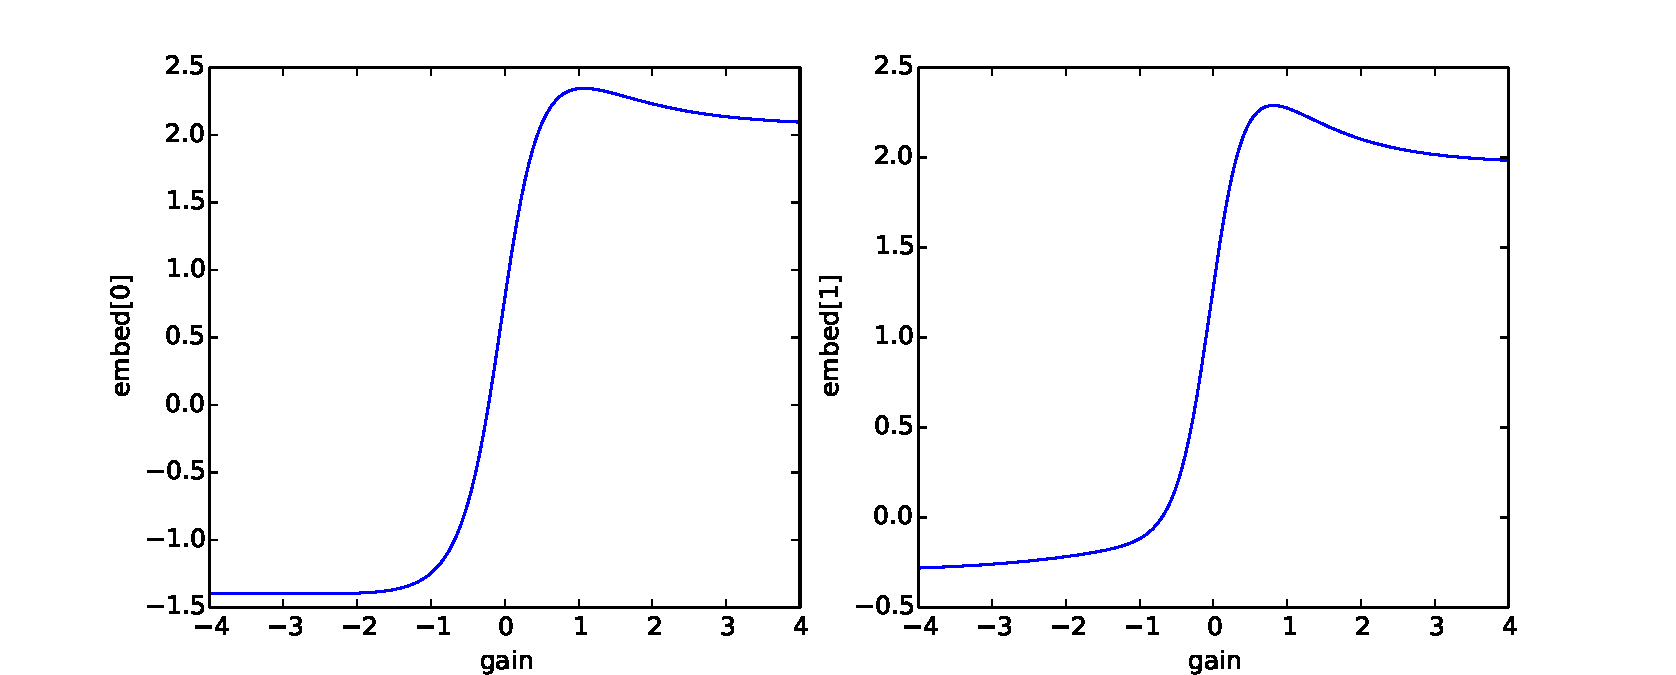
\includegraphics[width=\textwidth]{pointmass_embed_mapping.pdf}
\caption{
Learned mapping from gain factor $g$ to two-dimensional embedding space in point-mass environment.
}
\label{fig:embed-mapping}
\end{figure}
Figure~\ref{fig:embed-mapping} shows the learned mapping from the gain factor $g$
to the embedding space $\cL$.
\TODO{interpret.}

\begin{figure}
\centering
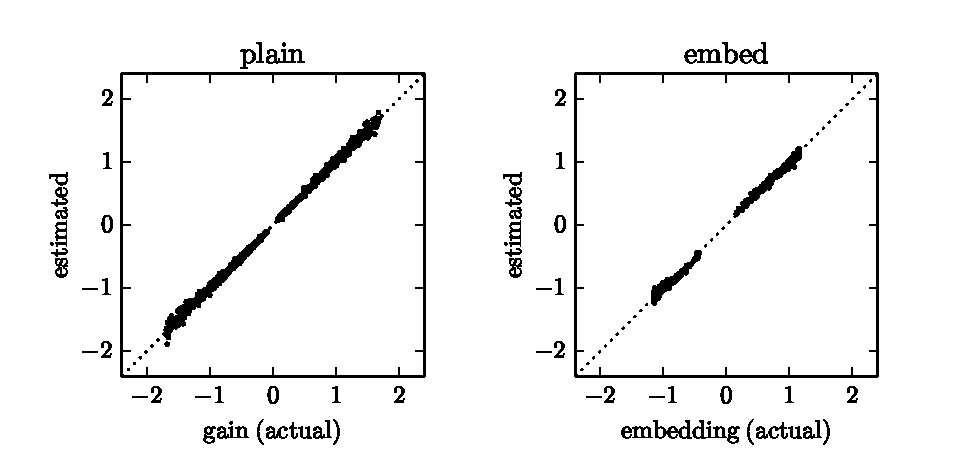
\includegraphics[width=0.85\textwidth]{pointmass_embed_scatter.pdf}
%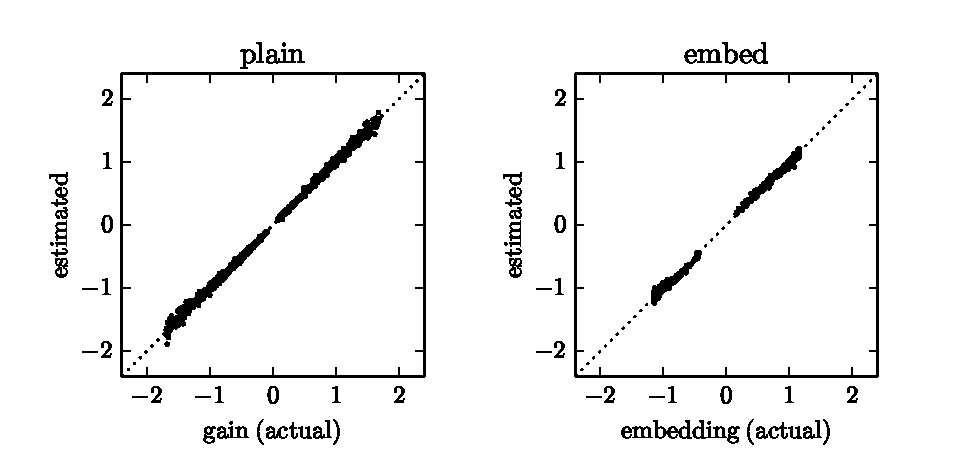
\includegraphics[width=0.45\textwidth]{pointmass_embed_scatter.pdf}
\caption{Scatter plots of actual vs. estimated SysID values.
\emph{Left:} gain parameter $g$ with ``plain'' policy.
\emph{Right:} one of two learned embedding dimensions with ``embed'' policy.
The embedding network separates the gain values into positive and negative clusters.
}
\label{fig:scatter}
\end{figure}
The scatter plots in figure~\ref{fig:scatter} compare the ground truth embedding values gainst those estimated by the inference network in \emph{our} policy, and for the gain factor $g$ against the values estimated by the SysID network in the \emph{plain} policy.
%Against the $x-$axis, density estimates are shown.
These plots illustrate that the learned embedding function ``squashes'' the gain factor $g$ into positive and negative clusters.
The separation between these clusters is magnified, making it easier for the policy to switch between two disjoint behavior styles depending on the sign of the gain factor.
\TODO{can we say anything less wishy-washy? how can we back up this claim?}

\begin{figure}
\centering
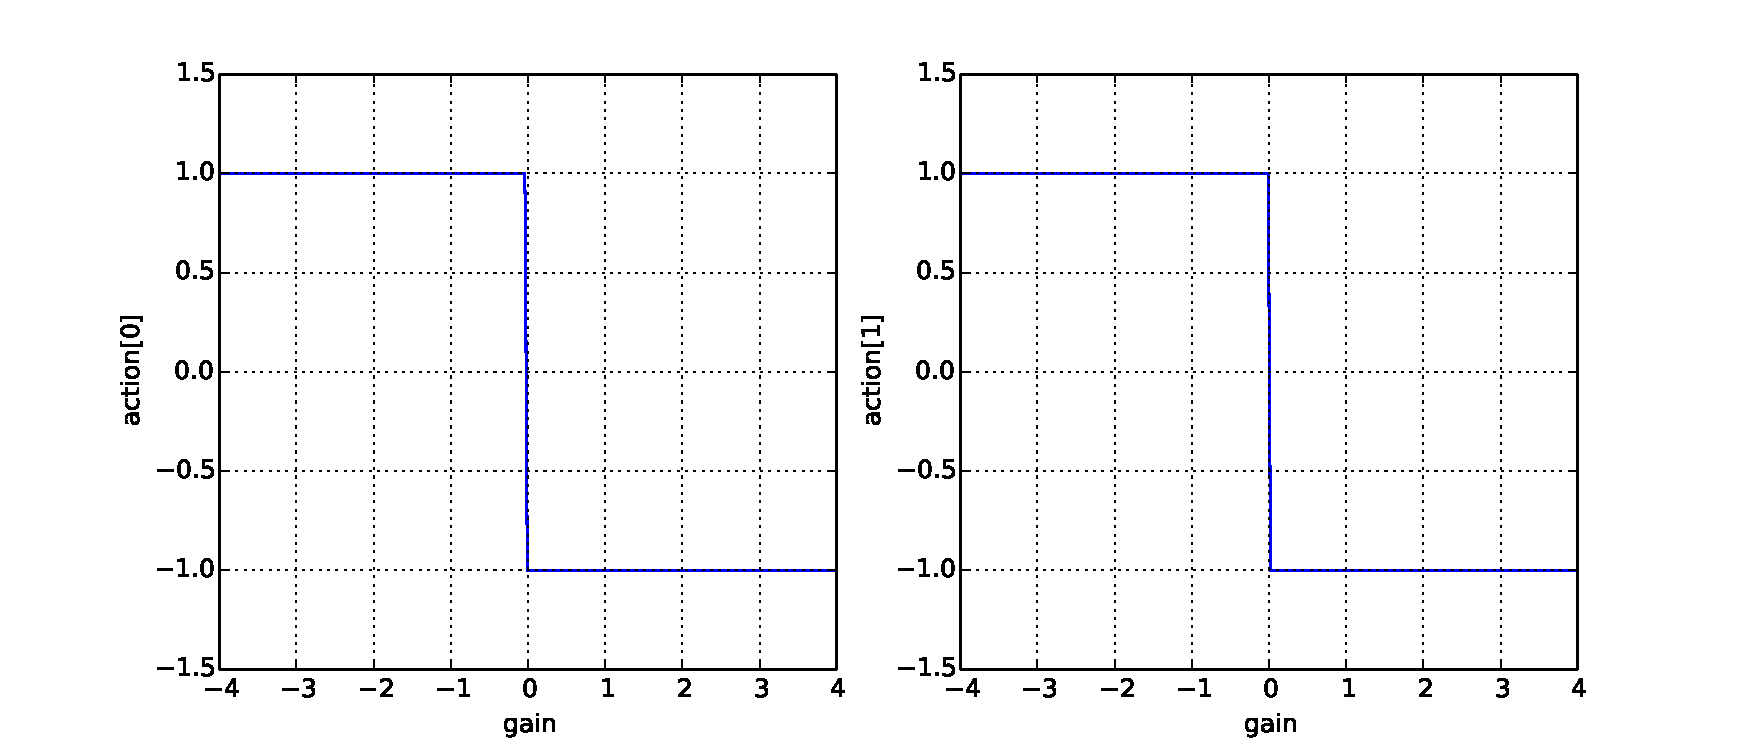
\includegraphics[width=\textwidth]{pointmass_conditional_action.pdf}
\caption{
Action of trained \embed{} policy at initial state (position $ = (1,1)$, velocity $=(0,0)$) conditioned on gain factor $g$.
Outputs are clipped to valid action range.
Plots show that policy has learned the optimal bang-bang control policy in both positive and negative gain scenarios.
}
\label{fig:conditional_action}
\end{figure}

Figure~\ref{fig:conditional_action} shows the policy output $\pi(a|s_D)$ conditioned on
the gain factor $g$ at the initial task state $s_{t0} = (1, 1)$.

\subsubsection{Disentangling of redundant features}

\begin{figure}
\centering
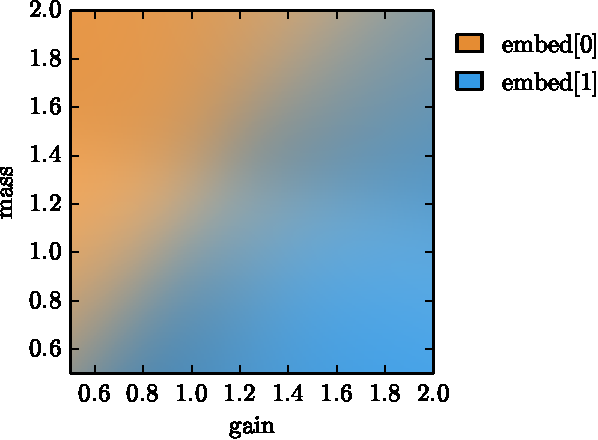
\includegraphics[width=0.5\textwidth]{embed_colors.pdf}
\caption{
Illustration of learned embedding space that disentangles redundant dynamics parameters.
Graph axes represent true dynamics parameters; colors represent learned embedding values.
In point-mass environment with parameters of gain $g$ and mass $m$,
the dynamics only depend on the $g/m$ ratio.
The learned embedding reflects this; for example, the $g=m$ line is all mapped to similar embedding values.
}
\label{fig:embed_colors}
\end{figure}
A primary benefit of our approach is its ability to distill potentially complex sets of dynamics parameters
into a simplified space where only the minimal information needed to achieve good rewards is preserved.
We illustrate this by constructing a version of the point-mass environment with redundant features:
we add a mass parameter $m$ alongside the gain parameter $g$.
Now, the true force applied to the mass is proportional to $g/m$,
making all $(g, m)$ combinations with the same ratio indistinguishable to system identification.
This poses a problem for the \plain{} or \extra{} frameworks
because the learning problem of recovering the true $(g, m)$ from a state-action trajectory is ill-posed.
In contrast, our framework learns an embedding where all $(g, m)$ combinations with similar ratios are mapped to similar embedding values.
This embedding is visualized in Figure~\ref{fig:embed_colors}.

\begin{comment}
\begin{figure}
\centering
\TODO{learning curves for redundant point-mass.}
\caption{
Example of incompatibility between our observability objective \TODO{ref}
and attempting to reconstruct the true dynamics parameters
in redundant point-mass environment.
When $\alpha = 0.1$, \extra{} network alters its behavior in pursuit of the observability reward, but the dynamics parameters are impossible to estimate.
The learning process is disturbed.
When $\alpha = 0$, \extra{} network does not alter its behavior
and learns a policy that accounts for the many-to-many characteristic of the estimation problem.
}
\label{fig:redundant_fail}
\end{figure}
\end{comment}


Note that the learned embedding in these examples is two-dimensional -- 
the operator does not need to know the minimal dimensionality of the parameters after redundancies are removed.
This is important in scenarios with many parameters where identifying redundant parameters 
is not as simple as in the point-mass environment.

\subsection{More Complex Environment}

\begin{figure}[h]
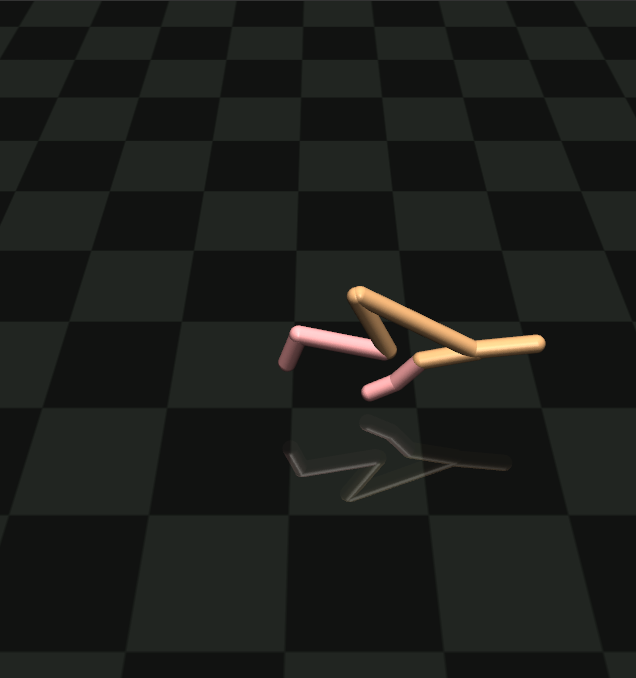
\includegraphics[trim=4cm 3cm 0cm 4cm, clip, width=0.22\textwidth]{cheetah_short.png}\hfill
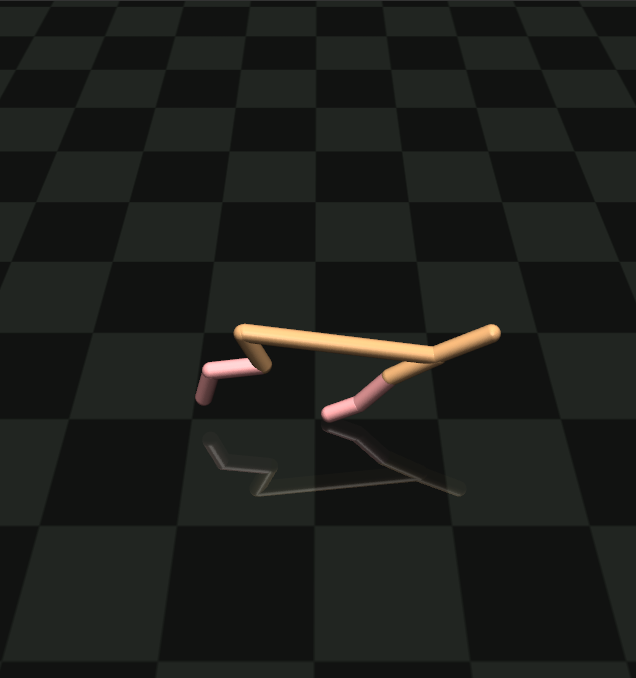
\includegraphics[trim=4cm 3cm 0cm 4cm, clip, width=0.22\textwidth]{cheetah_medium.png}\hfill
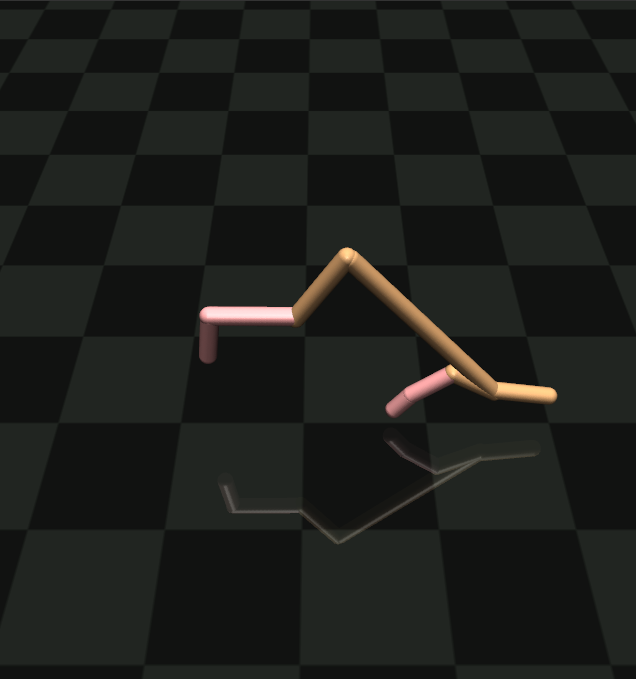
\includegraphics[trim=4cm 3cm 0cm 4cm, clip, width=0.22\textwidth]{cheetah_backleg.png}\hfill
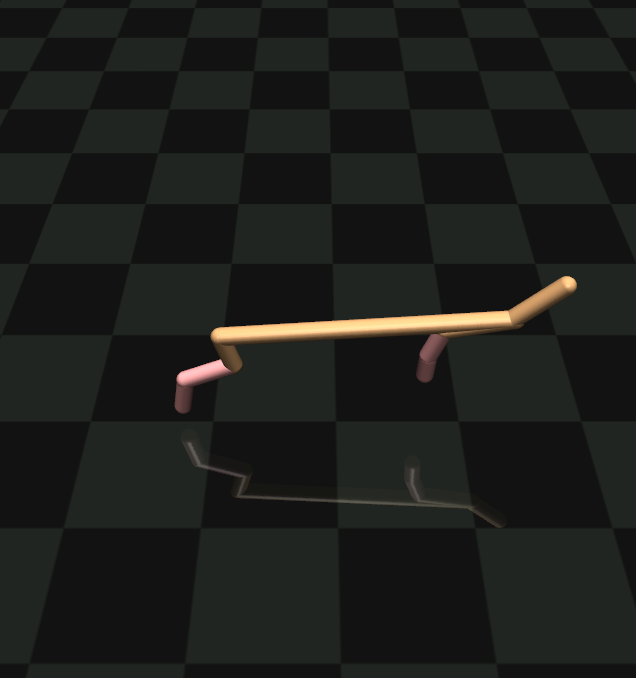
\includegraphics[trim=4cm 3cm 0cm 4cm, clip, width=0.22\textwidth]{cheetah_long.png}
\caption{Variations of Half-Cheetah environment produced by randomization of kinematic and dynamic properties.}
\label{cheetahs}
\end{figure}

As an example of a more complex task, we demonstrate results on the \emph{Half-Cheetah}
planar locomotion environment from the OpenAI Gym~\citep{openai-gym}.
The following parameters are randomized:
lengths of seven kinematic links,
damping, stiffness, and ranges of six planar revolute joints,
and gear ratios of six rotary actuators.
In total, 37 parameters are randomized.
The embedding space $\cL$ is 8-dimensional.
Each end of the joint range is shifted by $\pm 0.3$ radians.
All other parameters are multiplied by a ratio log-uniformly distributed in the range $[0.57, 1.75]$.

Due to the architecture of the MuJoCo physics simulator used in this environment~\citep{todorov-mujoco},
it is not practical to sample new random dynamics parameters $s_D$ for each training iteration.
Instead, we construct a ``universe'' of 256 models initially, and randomly choose 8 of these environments for each training iteration.
At test time, we resample a new ``universe'' of models.

Preliminary results from these experiments are showin in~\figref{cheetah-boxplot}
The experiments demonstrate that the learned embedding space helps to achieve higher rewards
compared to estimating the dynamics properties directly.
(comparison with \blind{} coming soon.)

\begin{figure}[h]
\centering
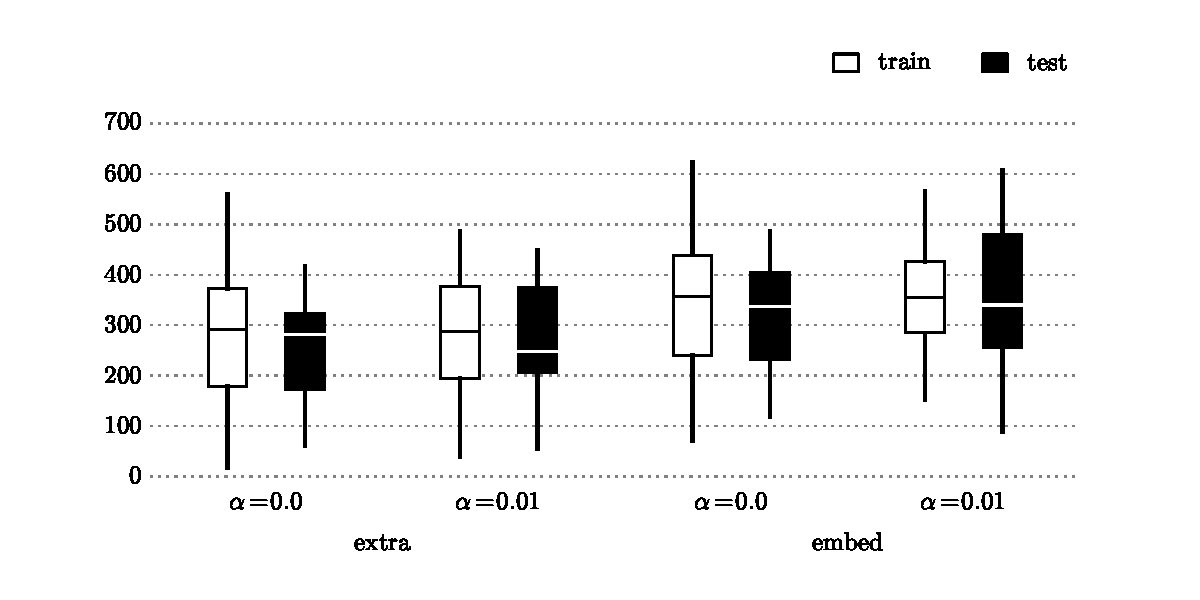
\includegraphics[width=\textwidth]{halfcheetah_rewards.pdf}
\caption{
Box plots of training and test rewards in half-cheetah environment for \extra{} and \embed{} policies.
Learned embedding space gives significant improvement.
Observability reward $\alpha$ gives moderate improvement.
}
\label{cheetah-boxplot}
\end{figure}


\subsection{Architecture and Implementation Notes}
\label{implementation}
In all experiments, we use Proximal Policy Optimization (PPO)~\citep{schulman-ppo} as our reinforcement learning algorithm.
The policy $\pi$ is parameterized as a fully connected neural network with 3 hidden layers of 128 units each, using ReLU nonlinearities.
The advantage function used as a baseline by PPO uses an identical network.
The embedding function $\embedfn$ network contains 2 hidden layers with 74 units each.
The system identification function $\idfn$ is composed of 3 convolutional layers followed by 2 fully-connected layers.


\section{Conclusion}
In this paper, we demonstrated a novel framework for training robot control policies
that can adapt online in real time to variations in system dynamics parameters.
We learn an embedding space that distills the full system identification information
and can disentangle redundant and unobservable parameters, while providing only the information that is useful for decision making.
We introduce an observability reward function in the reinforcement learning reward,
such that the control policy is encouraged to behave in a way that makes system identification easier.
Experimental results illustrate the desirable properties of the embedding space on a low-dimensional problem
and demonstrate improved training performance and test generalization compared to baselines
where the embedding space and observability reward are not used.
Future work will focus on applying this method to simulation-to-reality transfer on a real robot.

\clearpage
\acknowledgments{}
\bibliography{bibliography}{}

\end{document}
